\documentclass[twocolumn]{el-author}

\usepackage[utf8]{inputenc}
\usepackage{graphicx}

\date{31 octobre 2025}

\begin{document}

\title{Solution à la problématique de labellisation d'images de plaques d'immatriculation floues dans Label Studio}

\author{Membres du laboratoire de recherche en IA}

\abstract{Ce rapport présente une problématique rencontrée lors de la labellisation d'images de plaques d'immatriculation dans Label Studio, ainsi que la stratégie développée pour y remédier. La difficulté principale résidait dans le flou excessif de certaines images en pleine résolution, rendant impossible l'identification et la délimitation précise des caractères alphanumériques. Nous avons observé que les miniatures de ces mêmes images présentaient paradoxalement une meilleure lisibilité. Cette observation nous conduit à utiliser les miniatures comme guides visuels pour la labellisation des images floues sur Label studio.}

\maketitle

\section{Introduction}

La labellisation d'images de plaques d'immatriculation constitue une étape cruciale dans le développement de systèmes de reconnaissance automatique de plaques. Le processus consiste à délimiter précisément chaque caractère (chiffres et lettres) présent sur la plaque à l'aide de boîtes englobantes (bounding boxes). Cette tâche nécessite une visibilité claire de chaque caractère pour garantir la précision des annotations.

% INSÉRER ICI : Capture d'écran d'une image de plaque correctement visible dans Label Studio avec des boîtes englobantes autour de quelques caractères pour illustrer le processus normal de labellisation
% \begin{figure}[h]
% \centering{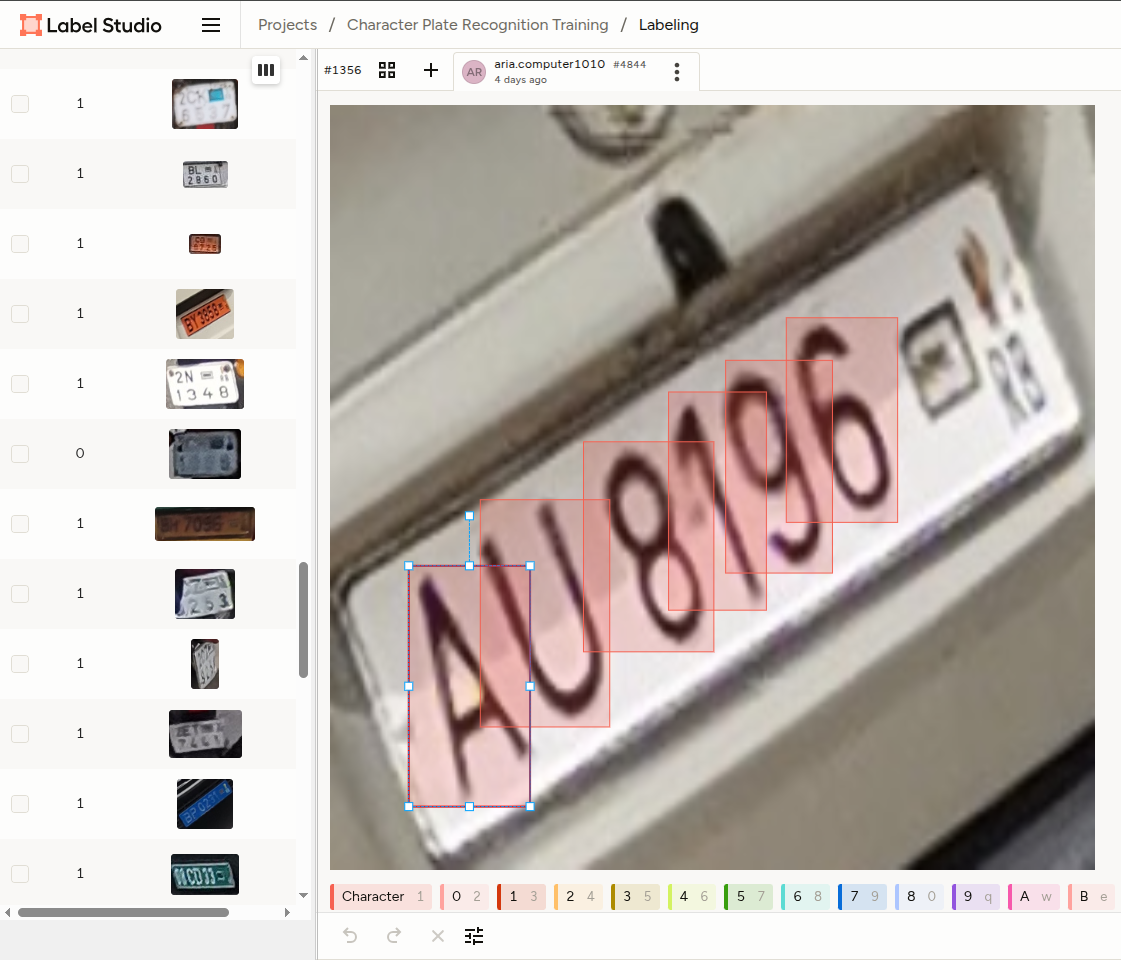
\includegraphics[width=85mm]{image_plaque_normale}}
% \caption{Exemple de labellisation normale d'une plaque d'immatriculation dans Label Studio. Chaque caractère est entouré d'une boîte englobante.}
% \end{figure}

\section{Problématique rencontrée}

Lors de nos travaux de labellisation dans Label Studio, nous avons été confrontés à une difficulté majeure : un nombre significatif d'images de plaques présentaient un flou excessif lorsqu'elles étaient affichées en pleine résolution dans l'interface de labellisation de Label Studio. Ce flou rendait les caractères alphanumériques pratiquement illisibles, comme illustré dans la Figure 2.

L'impossibilité de distinguer clairement les caractères compromettait l'exactitude de la labellisation, car il devenait extrêmement difficile, voire impossible, de déterminer les limites précises de chaque lettre ou chiffre. Cette situation risquait de produire des annotations de mauvaise qualité, ce qui aurait des répercussions négatives sur l'entraînement de modèles de reconnaissance de plaques.
Pour cela, on était obligé de sauter ces images. Et résultat notre modèle final avait des difficultés à lire les plaques d'immatriculation se trouvant de loin sur une photo.

% INSÉRER ICI : Capture d'écran d'une image de plaque floue affichée en pleine résolution dans Label Studio, montrant l'impossibilité de distinguer clairement les caractères
% \begin{figure}[h]
% \centering{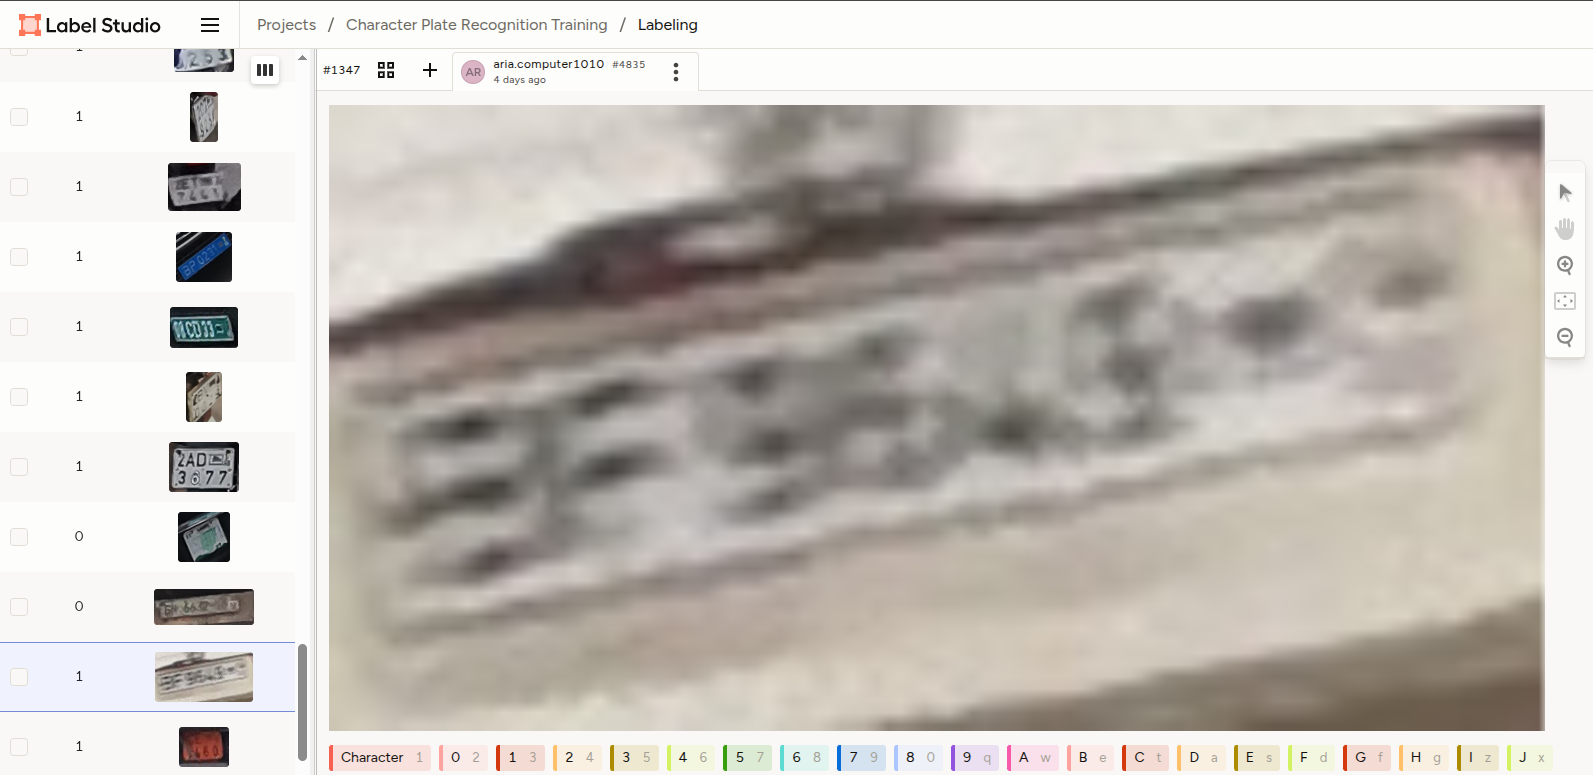
\includegraphics[width=85mm]{image_plaque_floue_fullsize}}
% \caption{Image de plaque floue affichée en pleine résolution dans Label Studio. Les caractères sont difficilement identifiables en raison du flou important.}
% \end{figure}

\section{Observation et solution proposée}

Face à cette problématique, nous avons effectué une observation inattendue : en examinant ces mêmes images floues sous forme de miniatures (thumbnails), les caractères apparaissaient paradoxalement plus lisibles et identifiables que sur l'interface de Label Studio. Cette meilleure visibilité en miniature peut s'expliquer par l'effet de réduction d'échelle qui atténue visuellement le flou et améliore le contraste apparent entre les caractères et l'arrière-plan.

% INSÉRER ICI : Capture d'écran côte à côte ou comparative montrant la même plaque en miniature (plus lisible) et en pleine résolution (floue)
% \begin{figure}[h]
% \centering{\includegraphics[width=85mm]{comparaison_miniature_fullsize}}
% \caption{Comparaison entre la miniature (à gauche, caractères plus visibles) et l'image en pleine résolution (à droite, caractères flous).}
% \end{figure}

Cette découverte nous conduit à élaborer une méthode de travail alternative : utiliser la version miniaturisée de l'image comme référence visuelle pour guider la labellisation sur l'image en pleine résolution. Concrètement, l'annotateur consulte la miniature pour identifier la position et la nature de chaque caractère, puis reporte ces informations sur l'image en haute résolution dans Label Studio en plaçant les boîtes englobantes aux emplacements correspondants.

\section{Mise en œuvre pratique}

La méthode proposée nécessite l'affichage simultané de la miniature et de l'image en pleine résolution dans Label Studio. L'annotateur procède selon les étapes suivantes :

\begin{enumerate}
\item Ouvrir l'image floue dans Label Studio pour la labellisation
\item Afficher la miniature de cette même image dans une fenêtre adjacente ou sur un second écran
\item Identifier les caractères sur la miniature
\item Reporter les positions approximatives sur l'image en pleine résolution en traçant les boîtes englobantes
\item Ajuster les délimitations en tenant compte de la structure générale de la plaque
\end{enumerate}

% INSÉRER ICI : Capture d'écran montrant le processus de labellisation avec la miniature comme guide (peut montrer les deux fenêtres côte à côte ou une capture annotée expliquant le workflow)
% \begin{figure}[h]
% \centering{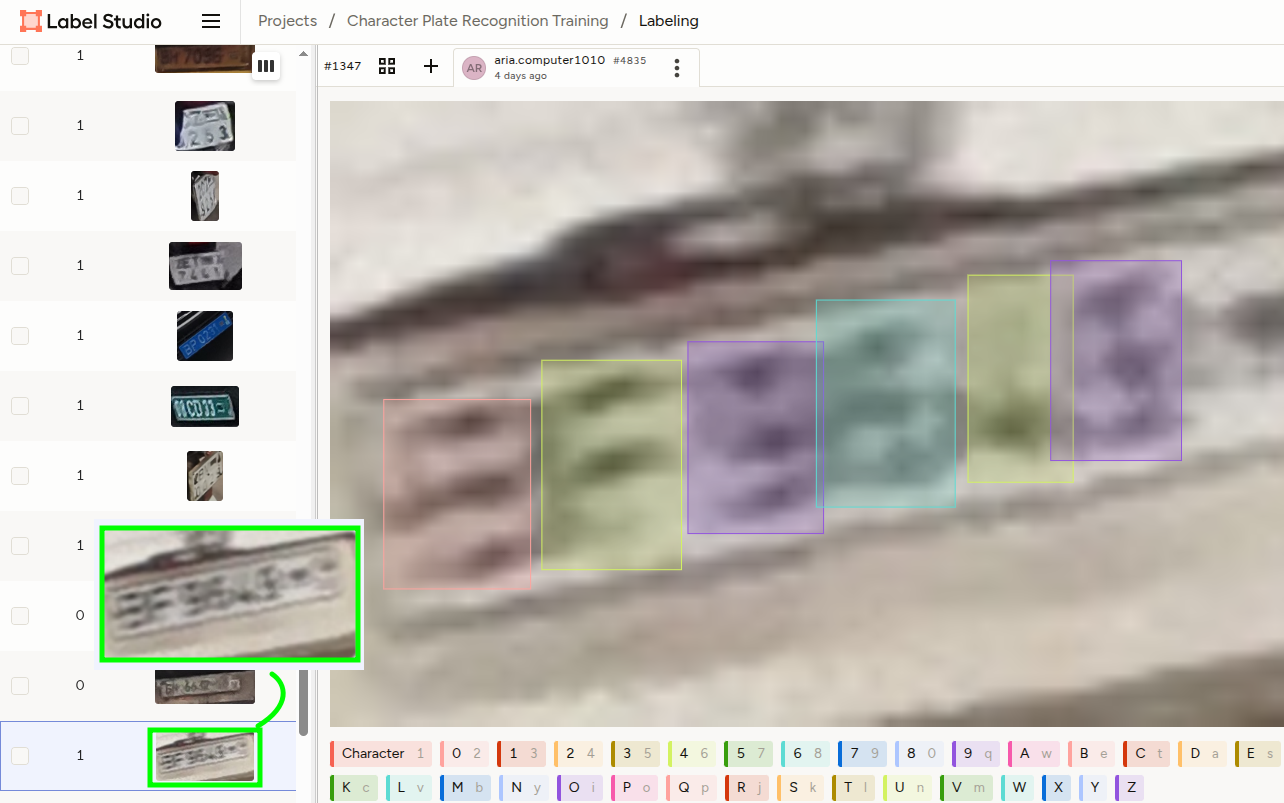
\includegraphics[width=85mm]{processus_labellisation_guide}}
% \caption{Processus de labellisation utilisant la miniature comme guide visuel. L'annotateur identifie les caractères sur la miniature (référence) avant de les labelliser sur l'image en pleine résolution.}
% \end{figure}

Cette approche permet de maintenir une qualité de labellisation acceptable même pour des images de qualité médiocre, tout en évitant de rejeter systématiquement ces images du jeu de données d'entraînement.

\section{Conclusion}

Nous avons identifié et résolu une problématique significative dans le processus de labellisation d'images de plaques d'immatriculation floues. L'utilisation des miniatures comme guides visuels constitue une solution pragmatique qui permet de valoriser des images qui auraient autrement été inexploitables. Cette méthode améliore l'efficacité du processus de labellisation et permet d'enrichir le jeu de données avec des exemples variés, y compris des images de qualité sous-optimale, ce qui peut contribuer à la robustesse des modèles entraînés.

% \ack{Nous remercions l'équipe technique pour son soutien dans la résolution de cette problématique.}

\vskip5pt

\noindent Membres du laboratoire de recherche en IA (\textit{UATM GASA FORMATION})
\vskip3pt

\noindent E-mails : dr.mokira@uatmgasa.com, info@uatm-gasa.com
\vskip5pt

\noindent Date : \today

\end{document}